% This is the LaTex template file for the Journal "Language Development Research"
% Version: 1.0 (2022)
% Author: Mitja Nikolaus (mitja.nikolaus@posteo.de)
% Compile this file using pdflatex.
% The repository for the source files can be found at
%
%     https://github.com/mitjanikolaus/ldr-template
%

\documentclass{ldr-article}
%\usepackage{biblatex}
%\addbibresource{main.bib}

% here we can set the page counter to the correct global page counter
\setcounter{page}{1}

% Here we can set the correct volume and issue number for accepted articles
\fancyfoot[C]{\titlepagefontsize Volume X, Issue Y, 23 June 2023}


\title{A proof-of-concept process for validated brain emulation boot-strapped on an in-silico fully known ground-truth neural circuit}


\author{
Randal A. Koene\\
Thomas Liao\\
Carboncopies Foundation for Brain Research (Should this say 'Substrate Independent Minds' instead?)\\
(Also, is it in the right place?)
}

\def\firstexp{\textit{e0\_bs} }

\begin{document}

    \maketitle

    \begin{abstract}
       (This will need to be re-written... the text here is temporary.)
       There is presently not a single published proof-of-concept example where a process of brain emulation has been carried out at some scale and where a validation was performed to quantify the degree to which an emulation satisfies necessary success criteria. Scientific motivation to make progress in brain emulation depends on having a touch-stone implementation and reference evaluation to quantitatively improve upon. The only way to evaluate claims of brain emulation is through the use of metrics that compare an emulation with an original system. Similarity metrics must measure similarity in ways that matter to the goal of whole brain emulation, i.e. that satisfy cognitive success criteria. E.g. spike train timing is not duplicated, but the probability of spiking is modulated sensibly and the evolution of system attractors is plausible. Similarity metrics are needed at multiple levels and while some can be used only with fully known ground-truth systems, others will carry over to whole brain systems. The principle of brain emulation depends on the ability to satisfy cognitive success criteria while replacing implementation details at some scale. In analog, potentially chaotic systems, scale separation is achieved through the application of operational constraints. E.g. rhythms (brain) or clock cycles (computer), neural population activity (brain) or parity bits (computer), action potentials (brain) or binary thresholds (computer). The application of constraints at consecutive levels limits the size of each black box in system identification.
    \end{abstract}
    
    \keywords{brain emulation; system identification; similarity metrics; in-silico}
    \correspondingauthor{Randal A. Koene, CSO, Carboncopies Foundation for Brain Research, Sacramento, CA, and Nextup Neuro, LLC, Email: rkoene@carboncopies.org.}
    \orcids{https://orcid.org/0000-1234-5678-9999; }
    % for multiple ORCIDs, use \orcids and URLs separated by semicolons, e.g.:
    %\orcids{https://orcid.org/0000-1234-5678-9999;https://orcid.org/0000-5678-1234-9999}
   % \citationinfo{Other, A.N., Kramer, W.K., \& Pierce, J. (2022). Article title goes here. \textit{Language Development Research, 2}(1), XX–XX. \url{https://doi.org/10.34xxx/xxxx-xxxx}}


% =================================================================================
% SECTIONS PART 1 - problem description (paradigm change and translation challenge)
% =================================================================================

\section{Introduction}

REWRITE THESE NOTES:

A field of neuroscience that is aimed at neural circuit function reconstruction in a way that extends beyond the requirements explored in systems neuroscience, cognitive neuroscience, or neuroinformatics.

A description of how most neuroscience goes about making hypotheses, making predictions, testing hypotheses, making claims.
Existing specializations have emphasized the use of computation for hypothesis testing in the context of fundamental but abstracted concepts.

A description of how computational models are used in most of neuroscience in that process.

A reference to Konrad Kording’s paper about the problem that neuroscience would have in trying to explain a microchip.

A description of the aim of reducing the abstraction level and increasing the resolution at which modeling takes place until computational reconstructions have the functional characteristics of a specific sample, animal or person. These aims include not just correlational predictions, but a complete mapping that describes how representations have “meaning” from step to step within the propagating activity of a system. And these aims include identifying subjective uniqueness, and being able to recreate that in prosthetic form.
A neuroscience of reconstruction must emphasize not just shared operational fundamentals but individually unique functional structure, such as that which enables retrieval of personal memories.

For this process, we can apply well known methods for the progression from data to insight to hypothesis to model at the highest resolution.

Above that, we are working in the realm of large, complex systems with emergent properties, where characteristics depend on applied constraints.

The problem of satisfactory derivation of model parameters from data, identification and application of constraints is unsolved, building specimen-specific large scale neural reconstructions is relatively new, although reconstruction of individual neurons has history (e.g. see BlueBrain papers).

The problem has similarities with those in AI, where complex features and behaviors expressed in real world data need to be captured in rigorous and validated algorithms.

REWRITE BELOW FOR PROPER STYLE AND LANGUAGE:

There is presently not a single published proof-of-concept example where a process of brain emulation has been carried out at some scale and where a validation was performed to quantify the degree to which an emulation satisfies necessary success criteria. Scientific motivation to make progress in brain emulation depends on having a touch-stone implementation and reference evaluation to quantitatively improve upon. The only way to evaluate claims of brain emulation is through the use of metrics that compare an emulation with an original system. Similarity metrics must measure similarity in ways that matter to the goal of whole brain emulation, i.e. that satisfy cognitive success criteria. E.g. spike train timing is not duplicated, but the probability of spiking is modulated sensibly and the evolution of system attractors is plausible. Similarity metrics are needed at multiple levels and while some can be used only with fully known ground-truth systems, others will carry over to whole brain systems. The principle of brain emulation depends on the ability to satisfy cognitive success criteria while replacing implementation details at some scale. In analog, potentially chaotic systems, scale separation is achieved through the application of operational constraints. E.g. rhythms (brain) or clock cycles (computer), neural population activity (brain) or parity bits (computer), action potentials (brain) or binary thresholds (computer). The application of constraints at consecutive levels limits the size of each black box in system identification.

% =================================================================================
% SECTIONS PART 2 - introduction to the data (e.g. the process that leads to the data)
% =================================================================================

% =================================================================================
% SECTIONS PART 3 - state of the art (many ideas, little validation/verification)
% =================================================================================

% =================================================================================
% SECTIONS PART 4 - proposing a solution (how validation and accelerating iterative improvement, competition of methods, are achieved in other domains)
% =================================================================================

% =================================================================================
% SECTIONS PART 5 - implementing the solution (competition on known ground-truth systems, WBE challenge, two essential components: 1 - success criteria expressed by validation metrics, 2 - fully known ground-truth systems needed for rigorous metrics and performance)
% =================================================================================

% =================================================================================
% SECTIONS PART 6 - the challenge taking process (with example)
% =================================================================================

% =================================================================================
% SECTIONS PART 7 - results and how to use them
% =================================================================================

% =================================================================================
% SECTIONS PART 8 - progression (ladder of sophistication, in-silico to in-vitro to in-situ)
% =================================================================================




(Here: A paragraph that explains why the first example uses two imaginary ball-and-stick neurons.)
The ball-and-stick example is intended to provide the simplest in-silico case with the smallest
number of variables to address while still demonstrating the full process and dependencies
chain for whole brain emulation (see Fig.~\ref{fig:dependencies-pyramid}). This is an opportunity to anchor the development of useful similarity metrics for brain emulation.

(Here: Describe the I-XI requirements in the pyramid figure. Remove the topic levels text from the figure and put that description in here instead.)

In the following sections, we describe the process (parts I through XI) with the aid of an example experiment, \firstexp, that is designed as a simplest case in-silico with the minimum number of variables that can demonstrate the process. The abbreviation "bs" stands for ball-and-stick, because the neurons have only a spherical soma and a single axon component.

% -------------------------------------
% HERE: Add a desxcription of the WBE Challenge, as per the Transvision talk. This can then be
%       rewritten and reformatted to create the proper flow between all the things that need to be
%       conveyed.
% -------------------------------------

% %%% Add rewritten from: https://docs.google.com/document/d/1cKPBagv6YdD0KzLB-7ykoYiedZeG27py9NpsjuBRThU/edit

% %%% Add rewritten from https://docs.google.com/presentation/d/1c-oTM1neFsgqYN-vGu04ZRI30pW9pO6PLMy2gPfRbE0/edit#slide=id.g2b111662fa3_0_25

\section{Known ground-truth: In-silico sample preparation (XI) and characterized physiology (IX and VII)}

(Here: A paragraph explaining how we equate characterized ephys and biological brain samples with VBP architecture and components.)


\subsection{Requirement IX: Establishing a set of virtual physiological components with well-characterized dynamics}

For the purposes of testing methods and metrics, within this virtual brain laboratory, we define both the \textbf{morphology} and \textbf{physiology} of virtual components that we declare to be our \textbf{ground-truth} about which we know everything. The components of the \firstexp ground-truth model are as follows:

\begin{itemize}
	\item The system comprises a set of brain regions.
	\item A brain region (\textit{BrainRegion}) has a specified geometric shape and specified physiological content in the form of neural circuits.
	\item The type of neural circuit defined in \firstexp is a linearly aligned ball-and-stick neural circuit (\textit{BS\_Aligned\_NC}), so called, because the morphology of the neurons is essentially a ball with a stick.
	\item A neural circuit consists of some number of cells. Each of the cells has a specified morphology, characteristic dynamic functions of the neuron, and connectivity established by specifying receptors between a pre- and post-synaptic cell.
\end{itemize}

In \firstexp, the morphology is specified as a spherical soma (\textit{BS\_Soma}) and a cylindrical axon (\textit{BS\_Axon}) of particular dimensions (Fig.~\ref{fig:KGT-architecture}). A location is specified on the morphology for each receptor (\textit{BS\_Receptor}).

\begin{figure}
	\centering
	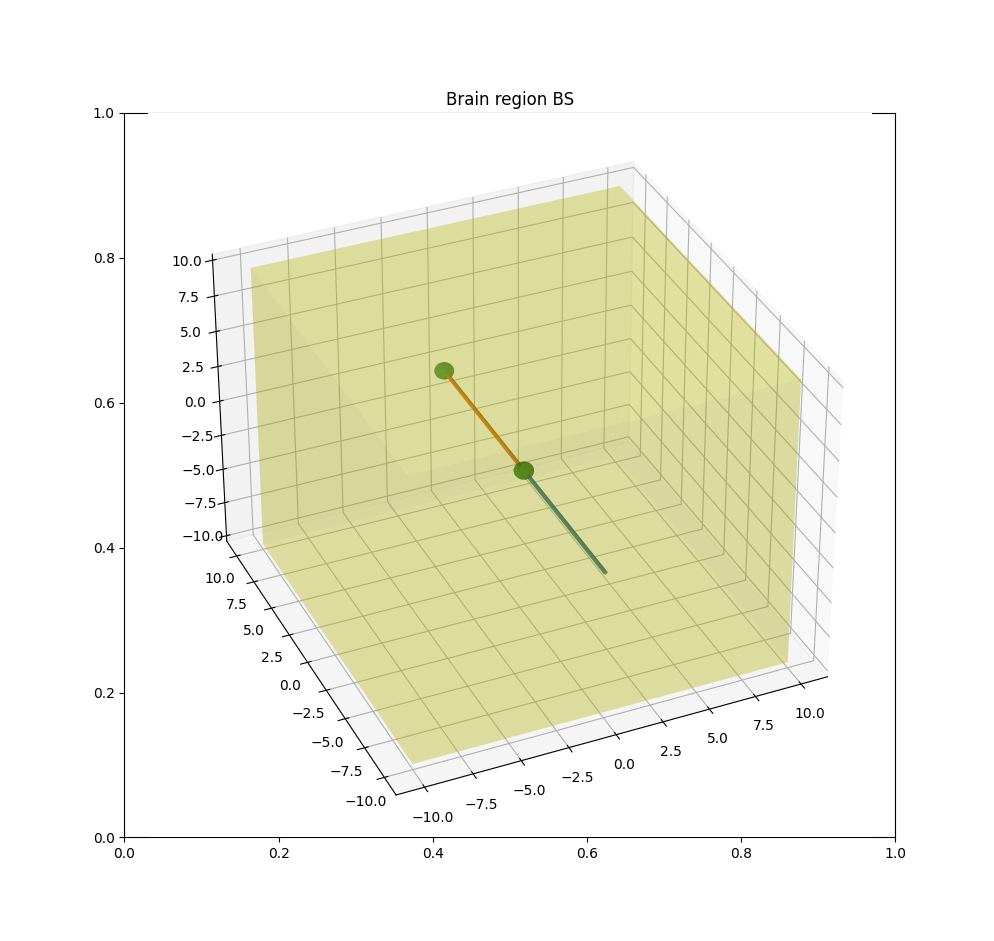
\includegraphics[width=1\linewidth]{figures/e0_bs.png}
	\caption{Diagram of the known ground-truth ball-and-stick neural circuit architecture within in-silico brain region.
	}
	\label{fig:KGT-architecture}
\end{figure}

Functional characteristics of each cell in \firstexp are specified by a neuron definition (\textit{BS\_Neuron}) and by weights associated with the synaptic receptors and their characteristic functions.

The \firstexp example is purposely extremely simple:
\begin{itemize}
	\item There is 1 brain region with a box shape, $20 \mu m$ on each side.
	\item The brain region contains a single neural circuit.
	\item That neural circuit has 2 neurons, one pre-synaptic, one post-synaptic.
	\item The neurons are identical, using the default parameter values for the ball-and-stick neuron class (\textit{BS\_Neuron}), see Table~\ref{tab:bs_neuron_default_pars}.
	\item The weight of the synaptic connection formed by a receptor has a value of $w_{syn} = 1.0$.
\end{itemize}

\begin{table}
	\begin{tabular}{ll}
		\centering
		Initial membrane potential & $V_m = -60 mV$ \\
		Resting membrane potential & $V_{rest} = -60 mV$ \\
		Action potential firing threshold & $V_{act} = -50 mV$ \\
		Spike potential during refractory period & $V_{spike} = 60 mV$ \\
		Time span of absolute refractory period & $\tau_{abs} = 1 ms$ \\
		After-hyperpolarization potential & $V_{AHP} = -20 mV$ \\
		After-hyperpolarization decay time constant & $\tau_{AHP} = 30 ms$ \\
		\hline
		Rise time constant of the post-synaptic potential & $\tau_{PSPr} = 5 ms$ \\
		Decay time constant of the post-synaptic potential & $\tau_{PSPd} = 25 ms$ \\
		Amplitude of the post-synaptic potential & $V_{PSP} = 20 mV$ \\
	\end{tabular}
	\caption{Default parameter values of ball-and-stick neuron class \textit{BS\_Neuron} and \textit{BS\_Receptor}.\label{tab:bs_neuron_default_pars}}
\end{table}

A simulation of activity in the ground-truth model carried out in small time increments (e.g. $1 ms$). For each neuron, the update function has two main steps:
\begin{enumerate}
	\item Update the momentary membrane potential, $V_m$.
	\item Detect threshold crossing and possibly generate a spike. This step is ignored if the neuron is still within the absolute refractory period, $\tau_{abs}$, of its most recent action potential.
\end{enumerate}

The momentary membrane potential is the sum of contributing potentials:
\begin{equation}\label{eq:membrane-potential}
	v_m(t) = V_{rest} + v_{spike}(t) + v_{AHP}(t) + \sum_i{v_{PSPi}(t)},
\end{equation}
where $v_{spike}(t) = V_{spike}$ during the absolute refractory period, and $v_{PSPi}(t)$ is the momentary post-synaptic potential contributed by the i-th receptor.

The refractory contribution of the spike:
\begin{eqnarray}
	v_{spike}(t) 	& = V_{spike} & \textrm{if } \Delta t_{act} \le \tau_{abs} \\
					& = 0 mV & \textrm{otherwise,} \nonumber
\end{eqnarray}
where $\Delta t_{act}$ is the time since onset of the most recent action potential.

Modulation of the membrane potential by after-hyperpolarization:
\begin{eqnarray}
	v_{AHP}(t)		& = V_{AHP} \exp(\frac{-\Delta t_{act}}{\tau_{AHP}}) & \textrm{if } \Delta t_{act} > \tau_{abs} \\
					& = 0 mV & \textrm{otherwise.} \nonumber
\end{eqnarray}

Post-synaptic contributions to the membrane potential caused by the propagation of pre-synaptic action potentials through input receptors:
\begin{eqnarray}
	v_{PSPi}(t)		& = w_{syn} V_{PSP} ( -\exp(\frac{-\Delta t_{act,i}}{\tau_{PSPr}}) + \exp(\frac{-\Delta t_{act,i}}{\tau_{PSPd}}) ) & \textrm{if the pre-synaptic neuron has spiked.} \\
					& = 0 mV & \textrm{otherwise,} \nonumber
\end{eqnarray}
where $\Delta t_{act,i}$ is the time since onset of the most recent action potential at the pre-synaptic neuron connected through receptor $i$.

A threshold crossing occurs if the new momentary membrane potential is at or beyond the firing threshold, $V_m \ge V_{act}$. If so, then a new spike onset time, $t_{act}$ is appended to the list of the neuron's spike times. That list is consulted by adjacent post-synaptic neurons that receive receptor input from this spiking neuron.

(Here: Mention how one would proceed on to the next more sophisticated step and towards working with real brain tissue for which there is no known ground-truth.)

\subsubsection{Requirement VII: In-silico representation of virtual brain components}

(Here: Describe preparation and use of the components library. Add reference to SW.)

\subsection{Requirement XI: Preparation of the virtual brain architecture of the known ground-truth system}

(Here: Describe how the architecture is set up. Add reference to SW. I.e. describe the steps that the model script takes to get to a defined known ground-truth system.)

\subsubsection{A virtual brain ground-truth system provides a ``God's eye'' record}

(Here: Describe how every calculated variable can be recorded for analysis and how that aids the development of similarity validation metrics.)

\begin{figure}
    \centering
    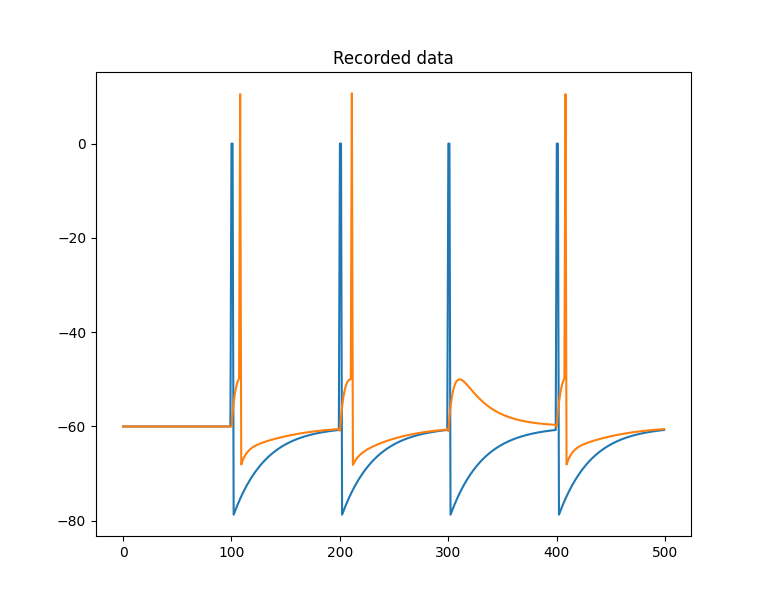
\includegraphics[width=1\linewidth]{figures/e0_bs_recorded.png}
    \caption{Plot of ball-and-stick neuron membrane potentials as recorded in ``God's eye'' mode during an experiment run.
}
    \label{fig:ball-and-stick}
\end{figure}

(Here: Make it clear that this is not the same as experimental data acquisition from the origin system.)

\section{Data acquisition: Double-blind experimentation in a virtual brain laboratory (X and VIII)}

(Here: Describe that even though the ground-truth model is fully known to the designer, the experimenter is blind to this and can use only data obtained through in-silico data acquisition that mirrors the process of data acquisition from biological brain systems.)

Simulated data acquisition is not permitted the God's eye view. Instead, it is constrained to the use of simulated data recording devices and simulated stimulation devices.

Activity observed is the result of either spontaneous simulated activity in the ground-truth system or activity caused by simulated stimulation methods. These may be simulated stimulation electrodes, simulated optogenetic stimulation, or others.

Typical simulated functional data recording devices include simulated recording electrodes of various types, simulated calcium imaging in a number of variants, or even simulated fNIRS or fMRI. In each case, detectable contributions of neuronal activity are combined with confouding factors (including noise, unreliability, defects) in simulation of the physics involved in measurements.

Typical simulated structural data recording devices include simulated microscopy of various types (e.g. electronmicroscopy, two-photon, light-sheet, etc). Again, the resulting images combine information about the ground-truth system morphology with confounding factors and effects of the physics involved.

Simulated data acquisition can be sophisticated and can attempt to model realistic results closely. Alternatively, simulated data acquisition can purposely apply simplifications for the following reasons:
\begin{enumerate}
	\item Ease and rapidity of implementation.
	\item Reduced computational cost.
	\item Producing simplified laboratory condition examples with fewer variables to consider.
\end{enumerate}
The simplified laboratory conditions reason is particularly useful, because this allows methods to be tested first in vastly simplified conditions where the capabilities and limitations of the method can be identified, demonstrated and evaluated in their most obvious form, without distracting contributors.

\subsection{Requirement X: In-silico experimental data acquisition}

(Here: Describe the data acquisition set up with the previously prepared KGT system and running data acquisition simulations. Add reference to SW.)

The steps of simulated data acquisition are:
\begin{enumerate}
	\item Initialize the ground-truth model (loading or rerunning the previous stage).
	\item Initialize simulated functional data acquisition by placing simulated electrodes or by setting up simulated calcium imaging.
	\item Run simulated data acquisition and store that functional data.
	\item Run simulated imaging by obtaining 2D projections of the 3D model and store that structural data.
\end{enumerate}

\subsubsection{Initializing simulated functional data acquisition}

In our example experiment, \firstexp, preparation of simulated functional data acquisition involves these steps:
\begin{enumerate}
	\item Specify expected spontaneous activity of the neurons in the system.
	\item Set up a simulated single recording electrode in a location approximately between the two neurons.
	\item Set up a simulated calcium imaging microscope that sees both neurons.
\end{enumerate}

To specify the expected spontaneous activity, we pick a mean spontaneous firing interval, $280 ms$, and its standard deviation, $140 ms$. This will be the same for both neurons in the example system. We call the \textit{set\_spontaneous\_activity()} member function with a list that associates the mean-stdev pair with each of the enumerated neurons.

A call to the \textit{attach\_recording\_electrodes()} member function is used to set up any number of simulated electrodes. In our example, we provide a list with the specifications for only one electrode. We provide the following specifications:
\begin{itemize}
	\item The position of the tip of the electode, at the geometric center of the system.
	\item The positions of recording sites on the electrode, in this case one site at the very tip.
\end{itemize}

Similarly, a call to the \textit{attach\_calcium\_imaging()} member function is used to set up a calcium imaging device. In \firstexp, we specify:
\begin{itemize}
	\item Both neurons will fluoresce and show up during imaging.
	\item We will use a simulated jGCaMP8 calicium indicator~(\cite{zhang2023}) with relatively fast and short response dynamics, specified by an indicator rise time of $2 ms$ and an indicator interval of $20 ms$.
	\item The lens front position is $(0, 20, 0)$, $20 \mu m$ above the simulated sample, and is positioned vertically, as indicated by a rear position $(0, 40, 0)$.
\end{itemize}

\subsubsection{Simulating functional data acquisition}

Simulated electrode and calcium imaging devices record data while we run the model for a specified number of simulated milliseconds.

(Here: put more about how those simulated devices generate the recorded data by using simulated physics.)


% Section about EM Rendering
\subsubsection{Simulating structural data acquisition}

We provide high-throughput microscope specifications:
\begin{itemize}
	\item Obtain images from the 'full' sample.
	\item The full sample is carved into sample sections $6 \mu m$ wide and long.
	\item Each image has $6000$ by $6000$ pixels.
	\item The voxel resolution (represented by each pixel) is $4 nm$ in x and y and $30 nm$ in the z dimension.
\end{itemize}

(Here: put more about how a simulated high-throughput EM image stack is generated using simulated optics.)

\begin{figure}
    \centering
    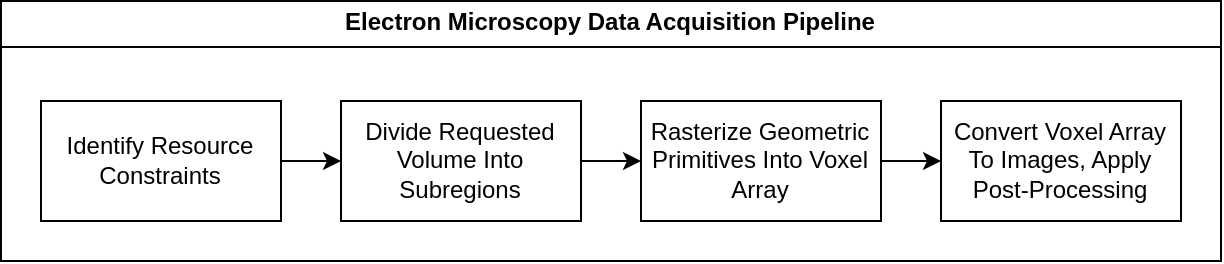
\includegraphics[width=1\linewidth]{Figures/VBP_EM_Render_Pipeline.drawio.png}
    \caption{High-level overview of the electron microscopy rendering process.}
    \label{fig:em-pipeline}
\end{figure}


Our approach involves three major steps. Firstly, we divide the volume into $n$ subregions, based on various system resource constraints. Next, we rasterize the geometric primitives used to represent the neural morphology in each subregion. Finally, the voxel array is traversed and converted to a 2D image array, post-processing applied, and saved.

% Todo: add detailed section describing each of these major steps
% Convert the above overview into a bullet-point based list
% Make a diagram showing the process? (maybe 3d, and have it show the voxel rasterization process? (better explainer than words))
% Also, describe some of the optimziations done and performance improvements
% Actually, the whole thing should be simplified a bit... (Don't include optimizations in the overview, add those in a subsection of this)
% right, that's all i think.



\subsection{Requirement VIII: Collected data and post-processing}

(Here: Describe what it means for the collected data to be the "relevant" brain data.)

(Here: Describe the format of data obtained and how it may be post-processed for this simple experiment. Add reference to SW.)

\section{System Identification and Translation to emulation model parameters (IV-VI)}

(Here: Explain what system identification is, model selection and structuring. Explain what Translation means, model fitting. Point out the importance of constraints and their application. Explain that this process can involve multiple concurrent attempts or repeated attempts, guided by the validation step and error identification.)

\subsection{Requirement VI: Model selection and structure derivation from activity data and morphological data (VI)}

(Here: Describe the process. Add reference to SW.)

\subsection{Requirement V: Application of constraints at multiple levels (V)}

(Here: Describe the process. Add reference to SW.)

\subsection{Requirement IV: Completing a process of system identification and translation for model architecture and parameters}

(Here: Describe the process. Add reference to SW.)

\section{Validation of candidate emulated systems using similarity and performance metrics based on success criteria for successful whole brain emulation (I-III)}

(Here: Describe similarity metrics that can be used in known ground-truth system and those that can be used in a broader category of systems, even biological brains. Explain that these will evolve as research proceeds from these most basic in-silico systems to more sophisticated systems.)

\subsection{Requirement III: Measuring similarity and performance}

(Here: Describe the application of metrics and the evaluation of results.)

\subsubsection{Using known ground-truth systems to develop methods for the identification of error sources and their correction}

(Here: Describe an example of an error and how its cause is determined. Describe how the system identification and translation is adjusted and the outcome improved. Add reference to SW.)

\subsection{Requirement II: Meeting success criteria}

(Here: Describe this important relationship.)

\subsection{Requirement I: Achieving a successful whole brain emulation for the ball-and-stick neural system}

(Here: Describe the outcome.)



% Section For How Our Software Backend Works
\section{Software Architecture (rephrase this later)}

(This also all probably needs to be rephrased later but here's something for now, just so we have something to show for it. I'm not really sure what the right tone to use here is so I'll try my best, but again, we *will* need to fix this later i think.)

(WHERE DID MY FIGURE GO!?!?!? WHY IS IT UP ABOVE THIS AND NOT RIGHT BELOW THIS MESSAGE?!?!?!?!)

\begin{figure}
    \centering
    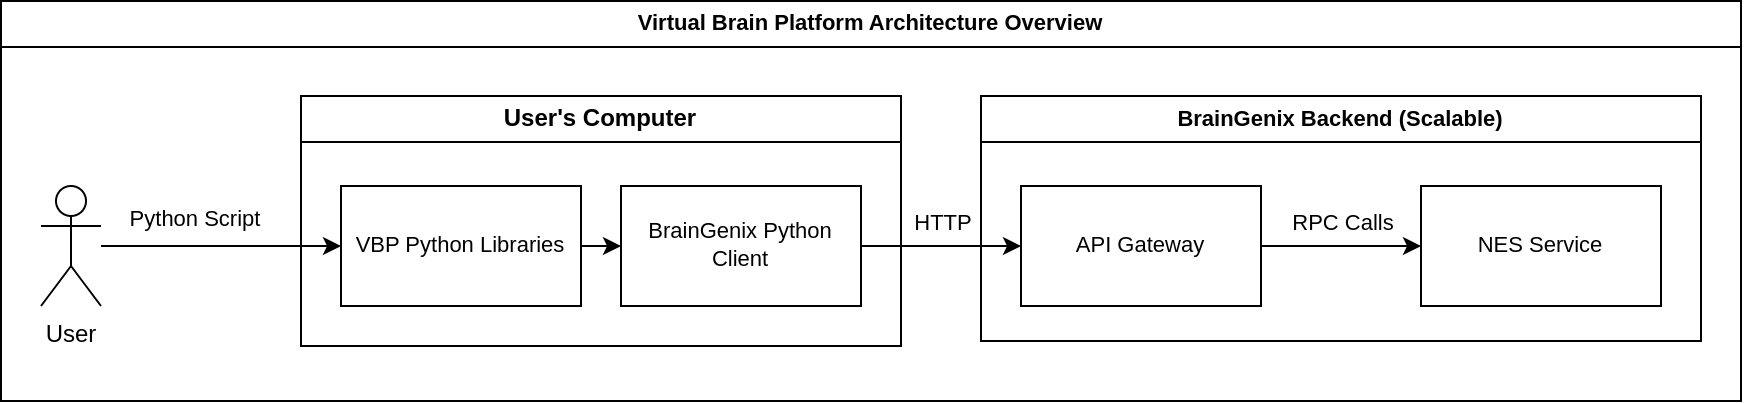
\includegraphics[width=1\linewidth]{Figures/VBP_System_Architecture_Overview.drawio.png}
    \caption{Diagram showing system architecture following a user's request.
}
    \label{fig:system-architecture}
\end{figure}

When designing the software system needed to generate the datasets, we elected to use a client-server based approach. This was done so out of concerns relating to performance and scalabillity. In future research, we envision generating significantly larger and more complex datasets, which would likely not fit on a single computer. To address this issue from the start, we focused on splitting the code in two places. On the client side, a simple python client library handles model definition and setup, while the backend resides on much more powerful servers.







\section{Discussion}

(Here: Discuss the main takeaways and important insights about the process for this simple system.)

(Here: Point to the follow-up research and the general procedure of step-wise advancement. Add a reference to the project and company.)

% Broken for now, disabling (due to same issue with biblatex, please fix dependencies Randal!)
%\printbibliography

\section{Data, Code and Materials Availability Statement}

(Here: Add links and DOIs to data, code and related materials.)

\section{Authorship and Contributorship Statement}

(Here: List who conceived the study, who designed the study and wrote the first draft of the manuscript. List other contributions. Mention if someone analysed data and revised the manuscript.)

All authors approved the final version of the manuscript and agree to be accountable for all aspects of the work in ensuring that questions related to the accuracy or integrity of any part of the work are appropriately investigated and resolved.

\section{Acknowledgements}

(Here: Add acknowledgments if applicable. This can include an acknowledgment of early support provided to the project.)

\clearpage
\appendix

\section{Appendices etc.}

(Here: Only if applicable.)

\end{document}
